\section{胶束}


\begin{frame}
    \frametitle{表面活性物质的临界胶束浓度}

    当表面活性物质浓度增至一定值，在表面层上，物质吸附达饱和，表面活性物质分子形成单分子层。表面层容纳不下的表面活性物质分子在溶液中以疏水基相互靠拢，形成以疏水基朝内、亲水基指向水相的胶束。形成胶束的浓度称为表面活性物质的临界胶束浓度，简称CMC，影响CMC的因素主要是分子的结构。
    \begin{figure}[htpb]
        \centering
        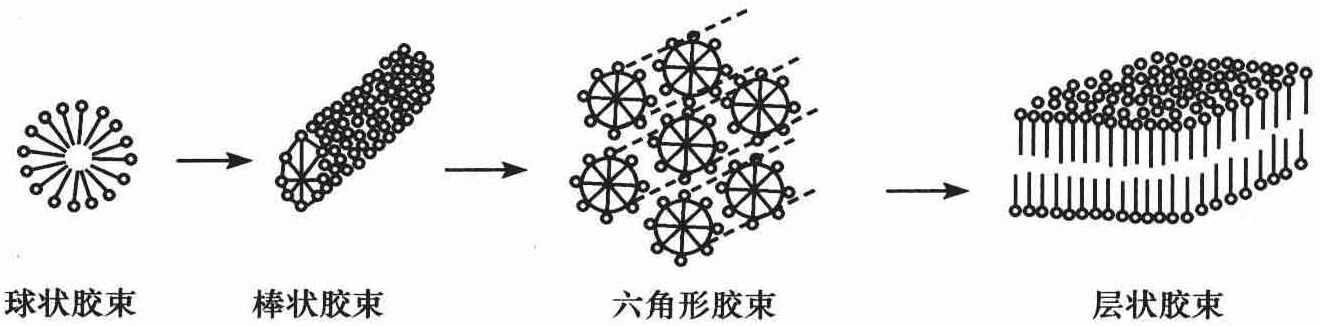
\includegraphics[width=.7\linewidth]{figures/fig8.12.png}
    \end{figure}
    \begin{itemize}
        \item 胶束的形状与形成胶束的浓度有关
        \item 胶束的大小与构成胶束的表面活性物质分子的数目即聚集数有关
    \end{itemize}

\end{frame}


\begin{frame}
    \frametitle{增溶作用}

    表面活性物质水溶液的一个重要应用，是能溶解一些原来不溶或微溶于水的物质。增溶作用的特征如下：
    \begin{enumerate}
        \item 增溶作用必须在CMC以上的浓度才能发生，即胶束的存在是发生增溶作用的必要条件，而且浓度越大，胶束越多，增溶效果越显著。
        \item 增溶作用是一热力学自发过程，可使被增溶物的蒸气压下降，化学势降低，增溶后体系更为稳定。
        \item 增溶后溶液为透明的体系，而且溶剂的依数性质基本不变。说明增溶并非溶解，溶质在增溶过程中并未在溶剂中分散成分子或离子状态，而是溶入胶束。溶液中质点总数未增加，只是胶束胀大。
        \item 增溶作用是一可逆的平衡过程。无论用什么方法，达到平衡后的增溶结果是一样的。
    \end{enumerate}

\end{frame}